\newcommand\variable{\emph{variable}\xspace}
\newcommand\variables{\emph{variables}\xspace}
\newcommand\widget{\emph{widget}\xspace}
\newcommand\widgets{\emph{widgets}\xspace}
\newcommand\constraint{\emph{constraint}\xspace}
\newcommand\constraints{\emph{constraints}\xspace}
\newcommand\Variable{\emph{Variable}\xspace}
\newcommand\Variables{\emph{Variables}\xspace}
\newcommand\Widget{\emph{Widget}\xspace}
\newcommand\Widgets{\emph{Widgets}\xspace}
\newcommand\Constraint{\emph{Constraint}\xspace}
\newcommand\Constraints{\emph{Constraints}\xspace}

\section{Contribution}

We assume that the reader is familiar with the complexity theory. In
this article, we will denote the set of instances by $\Omega$ and the
set of positive instances by $Y$. See the appendix for further
reminder on the complexity theory.

I did not manage to prove that the NST problem is NP complete. We will
also present in this section the different attempts we made and the
reasons why they were relevant but not conclusive. 

\subsection{Belonging to the NP class}

We aim to prove that the NST decision problem is NP-complete, this
means it would belong to the NP class and be NP-hard. It
clearly belongs to the NP class. Indeed, for all tree $T = (V,E)$, for
all integer $k$, given a potential solution $S$, it is possible to
ascertain whether or not $S$ is self-nested, and to compute the
distance between $S$ and $T$, both in polynomial time.

%%%%%%%%%%%%%%%%%%%%%%%%%%%%%%%%%%%%%%%%%%%%%%%%%%%%%%%%%%%%%%%%%%%%%%%%%%%%
\noindent\hrulefill

\subsection{First approach}
To help us build the reduction, a few conceptual remarks can be made,
in order to guide the research. First of all, the reduction has no
obligation to be surjective; as a matter of fact, it is quite often
not surjective. Indeed, in order to be able to prove the equivalence
$\omega_{A} \in Y_{A} \Leftrightarrow \omega_{B} = f(\omega_{A}) \in
Y_{B}$
(where $A$ is the initial NP-complete problem and $B$ is the problem
we consider), the images of the reduction have often a very
particular shape. Yet, the image of $\Omega_{A}$ by the reduction has
to be big enough so that we are unable to find a polynomial algorithm
solving the problem on the set of images of the reduction. Indeed,
finding such an algorithm and a reduction would mean we would have
solved the open question of the equality of the P and NP classes,
which is unreasonable.

In order to understand better the difficulty of the problem, I tried
to find a way to compute efficiently the NST in special cases. Indeed,
as long as we find a polynomial algorithm solving the NST problem on
the set of trees considered, we are ensured that the difficulty
leading to the NP-hardness lies somewhere else. I also decided to
start with very special cases where polynomial algorithms could be found
and to add progressively some generality to identify the trees and
conditions that make the problem difficult. 

I first considered the trees of height 2. In the NEST and NeST
algorithms, C. Godin, P. Ferraro and R. Azais consider only edit
operations such that the height of any pre-existing node is unchanged
(see Figure \ref{fig:edit_height}). For the sake of simplicity, I
decided to first use these edit operations.

\begin{figure}
  \centering
  \caption{edit operation height conservation}
  \label{fig:edit_height}
\end{figure}

\subsubsection{Trees of height 2 with height conservation} 
Let $T$ be a tree of height 2 (see Figure \ref{fig:height2}). Let us
denote $NST(T)$ by $S$ and an optimal edit mapping between $T$ and $S$
by $\Phi$. We will show in this section that it is possible to find
$\Phi$ and $S$ in polynomial time.  

We can first notice that if there are any leaves of depth 1, they do
not require any edit operations to obtain $NST(T)$. We can for this
reason assume that every node of depth 1 is of height 1 (see Figure
\ref{fig:height2}).

\begin{figure}
  \centering
  \includegraphics[width=.4\textwidth]{figures/tree_height2.pdf}

  \caption{example of tree of height 2}
  \label{fig:height2}
\end{figure}

Let us denote the nodes of height 1 of $T$ by
$(u_{i})_{1 \leqslant i \leqslant N}$ and
$(n_{i})_{1 \leqslant i \leqslant N}$ their respective number of
children. We will suppose that the sequence
$(n_{i})_{1 \leqslant i \leqslant N}$ is sorted by ascending
order. Each $u_{i}$ can be either deleted or mapped on a node of
height 1 in $S$, and since $S$ is self-nested, all the nodes of height
1 in $S$ are isomorphic to one another. The complete subtree under
each node of height 1 of $S$ is characterized by its number of
leaves. As a result, the edit mapping leading from $T$ to $S$ is
characterized by the $I_{0}$ the set of indices of the nodes deleted
and by $\tilde{n}$ the number of leaves under a node of height 1 in
$S$. Thus, we will try to find $I_{0}$ and $\tilde{n}$ such that the
corresponding self nested tree is a minimal distance from $T$.

Because of the constraint of Zhang, before deleting one of the nodes
$u_{i}$ of height 1 in $T$, it is necessary to delete all of his
children except one. Therefore, deleting $u_{i}$ costs $n_{i}$ where
$n_{i}$ is the number of children of $u_{i}$.

If $u_{i}$ is not deleted, than we have to adjust the number of
children it has to $\tilde{n}$, which costs
$\left|n_{i} - \tilde{n}\right|$. As a result, $u_{i}$ has to be
deleted if and only if $n_{i}$ is closer to 0 than to
$\tilde{n}$. Figure \ref{fig:optimalcost} shows $f_{i}$ the minimum
cost for each $u_{î}$ in function of $\tilde{n}$.

We will denote by $I_{1}$ the complement of $I_{0}$ in the set of
indices $\llbracket 1;N \rrbracket$. $I_{1}$ is composed of the
indices $i$ such that $\Phi(u_{i})$ is of height 1.
\begin{remark}
  The distance between $T$ and $S$ is equal to $\sum_{i \in I_{0}}
  n_{i} + \sum_{i \in I_{1}} \left| n_{i} - \tilde{n} \right|$
\end{remark}

\begin{figure}
  \centering
  \caption{optimal cost for $u_{i}$ in function of $\tilde{n}$}
  \label{fig:optimalcost}
\end{figure}

By summing the functions $f_{i}$ on every $u_{i}$, we obtain $f$ the
minimal cost of a mapping leading from $T$ to a self nested tree of
height 2, with $N$ nodes of depth 1, in function of $\tilde{n}$ the
number of children of the nodes of height 1. We can observe that the
resulting function is a piecewise linear function and that every break
in its differentiability has for abscissa one of the $n_{i}$ or
$2*n_{i}$. Therefore, the minimum of this function is reached in one
of those points. Since every $f_{i}$ is increasing just before
$2*n_{i}$ and constant after and that the derivative of the other
$f_{j}$ are equal before and after $2*n_{i}$, $2*n_{i}$ cannot be a
minimum of $f$.

Thus, by evaluating $f$ on every $n_{i}$, it is possible to find the
minimum of $f$ and thereby find the NST of $T$.

It is possible to show that every $f(n_{i})$ can be computed in
constant time by using the value of $f(n_{i-1})$. $f(n_{1})$ can be
computed in linear time. For this reason, $NST(T)$ can be computed in
$O(N*log(N))$ (it is necessary to order the
$(n_{i})_{1 \leqslant i \leqslant N}$ by ascending order) where $N$ is
the number of nodes of height 1 in $T$.

Since the NST (with only height preserving operations) can be computed
in polynomial time on the trees of height 2, this proves that if the
NST problem (with only height preserving operations) is NP-complete,
the set of images of the reduction cannot be the trees of height 2,
otherwise we would have found a way to solve any NP-complete problem
in polynomial time, which is unreasonnable.

We can make two more remarks that will help us later. 

\begin{remark} 
  For every $i \in I_{0}$, for
  every $j \in I_{1}$, $n_{i} < n_{j}$.\\
  Intuitively, if $n_{i} < n_{j}$ it costs less to delete all the
  children of $u_{i}$ than the one of $u_{j}$. See appendix for the proof.
\end{remark}

\begin{remark}
  Furthermore, $\tilde{n}$ is one of the medians of the
  $(n_{i})_{i \in I_{1}}$. \\
  Indeed, the median minimizes
  $\sum_{i \in I_{1}} \left| n_{i} - \tilde{n} \right|$. See proof in
  appendix for further details.
\end{remark}

We will keep in mind that the solution that we proposed here is a
brute-force search, we didn't manage to find any strategy that would
help us understand why computing the NST of a tree of height 2 seems
to be easier than in the general case. The main reason that explains
why this special case is easy to solve is that the trees of height 2
are simple enough to have a NST described by only 2 parameters.

\subsubsection{Trees of height 2 without preserving the height of the
  nodes}

The NST problem is solved easily on the trees of height 2 if we
authorize only the edit operations preserving the height. It can
either be due to the set of trees considered or to the restriction on
the edit operations. To gain in generality, I decided to look at the
problem without the restriction on the edit operations, in order to
use the work done in the previous section. Once again, I couldn't find
any global stategy that would give us a polynomial algorithm so I
tried to find as many properties on the NST of $T$ as I could, in
order to reduce the space of possibilities that we have to explore.

Since the poofs are quite fastidious we will only present the results
we found in this section, the poofs of the lemmas are in the appendix.

We will use the same notations as in the preceding paragraph. We will
denote by $I_{k}$ the set of indices $i$ of
$\llbracket 1;N \rrbracket$ such that $\Phi(u_{i})$ is of height
$k$. Let us denote by $\tilde{n}^{k}$ the number of children of the
nodes of height $k$ in $S$.

It is possible to show that $S$ has the shape depicted Figure
\ref{fig:shape_NST_2} %inserer figure
and that $S$ is characterized by
$(I_{k})_{0 \leqslant k \leqslant H-1}$ and
$(\tilde{n}^{k})_{1 \leqslant k \leqslant H-1}$ where $H$ is the
height of $S$. Therefore, the goal is to find the families
$(I_{k})_{0 \leqslant k \leqslant H-1}$ and
$(\tilde{n}^{k})_{1 \leqslant k \leqslant H-1}$ suh that the
corresponding self nested trees is at minimal distance from $T$.
\begin{figure}
  \centering
  
  \caption{Shape of $S$}
  \label{fig:shape_NST_2}
\end{figure}
The remarks of the previous section can be adapted.

\begin{lem}
  \label{lem:increasn}
  For every $k \geqslant 0$, for every $i \in I_{k}$ and $j \in
  I_{k+1}$, $n_{i} < n_{j}$.
\end{lem}

\begin{lem}
 The distance between $T$ and $S$ is equal to 
 $$ D(S,T) = \sum_{i \in I_{0}} n_{i} + \sum_{k = 1}^{H} \left(
   \sum_{i \in I_{k}} |n_{i} - \tilde{n}^{k}| + |I_{k}|\sum_{l =
     1}^{k-1}(\tilde{n}^{l}) \right)$$ 
 which is also equal to 
 $$ D(S,T) = \sum_{i \in I_{0}} n_{i} + \sum_{k = 1}^{H} \left(
   \sum_{i \in I_{k}} |n_{i} - \tilde{n}^{k}| + \tilde{n}^{k}\sum_{l =
     k+1}^{H}(|I_{l}|) \right)$$
 \begin{proof}
   Let $i \in I_{0}$. $u_{i}$ is deleted, which costs $n_{i}$ (as
   explained in the previous section).\\
   Let $i \in I_{k}$ with $k \geqslant 1$. $\Phi(u_{i})$ is of height
   $k$. To obtain the complete subtree under $\Phi(u_{i})$ in $S$ from
   the subtree under $u_{i}$ in $T$, it is necessary to adjust the
   number of children of $u_{i}$ to $\tilde{n}^{k}$ which costs
   $\left| n_{i} - \tilde{n}^{k} \right|$. It is also necessary to add
   $\sum_{l = 1}^{k-1}\tilde{n}^{l}$ nodes under one of the children
   of $u_{i}$, so that the height of $u_{i}$ increases to $k$.
   \end{proof}
\end{lem}

For every partition $(I_{k})_{0 \leqslant k \leqslant H-1}$ of
$\llbracket 1;N \rrbracket$, that verifies the lemma
\ref{lem:increasn}, it is possible to compute in $O(N)$ the family
$(\tilde{n}^{k})_{1 \leqslant k \leqslant H-1}$ such that the distance
between the corresponding self nested tree and $T$ is minimal. It is
also possible to show that

\begin{lem}
  \label{lem:ik}
  For every $k \geqslant 1$,
  $$|I_{k}| > \sum_{l = \ k+1}^{H-1} |I_{l}|$$
\end{lem}

\begin{lem}
  \label{lem:tilden}
  For every $k \geqslant 1$,
  $$\tilde{n}^{k} > \sum_{l = 1}^{k-1} \tilde{n}^{l}$$
\end{lem}
 
\begin{cor}
  The height $H$ of $S$ is bounded by $min(log_{2}(N+1),
  log_{2}(n_{N}+1))$.
  \begin{proof}
    The lemma \ref{lem:ik} leads to the following inequalities: 
    $$
    \begin{array}{rcl}
      |I_{k}| &\geqslant& \sum_{l=k+1}^{H} |I_{l}| + 1\\
              &\geqslant& |I_{k+1}| + \sum_{l=k+2}^{H} |I_{l}| + 1 \\
              &\geqslant& 2(\sum_{l=k+2}^{H} |I_{l}| + 1) \\
              &\geqslant& 2^{H-k-1}(I_{H} +1)\\
              &\geqslant& 2^{H-k}\\
    \end{array}
    $$
    As a consequence,
    $N \geqslant \sum_{k=1}^{H} |I_{k}| \geqslant \sum_{k=1}^{H}
    2^{H-k} \geqslant 2^{H} -1$,
    and $H \leqslant \left\lfloor \log_{2}(N+1) \right\rfloor$.\\
    The same reasonning can be applied to the lemma \ref{lem:tilden}
    to show that $H \leqslant \left\lfloor \log_{2}(\tilde{n}^{H}+1)
    \right\rfloor$, and we will notice that $\tilde{n}^{H} \leqslant
    n_{N}$, which leads to the result.
  \end{proof}
\end{cor}

By enumerating the partitions $(I_{k})_{0 \leqslant k \leqslant H-1}$
that verify the lemmas \ref{lem:increasn} and \ref{lem:ik} and
computing the optimal family
$(\tilde{n}^{k})_{1 \leqslant k \leqslant H-1}$ and the distance to
the corresponding self nested tree each time, we will find the NST of
$T$. The number of partitions $(I_{k})_{0 \leqslant k \leqslant H-1}$
of $\llbracket 1;N \rrbracket$ that verify the lemmas
\ref{lem:increasn} and \ref{lem:ik} is bounded by
$\frac{\binom{N+H}{H}}{2^H}$. 

Since $\frac{\binom{N+H}{H}}{2^H}$ is a $O(N^H)$ and that $H \leqslant
log_{2}(N)+1$, the number of partitions that have to be considered is
in the range of $N^{log_{2}(N)}$, which is unfortunetely not
polynomial.

I was not able to find any better compexity than this one, yet a few
remarks can be made. First of all, the complexity is expressed in
function of $N$ the number of nodes of height 1 and not in function of
the size of the tree and in practice, the trees that have a NST of
height close to the boundary $log_{2}(n)$ are very big in comparison
of $N$. Secondly, the proofs are far more complicated when all the
edit operations are considered than when only the height conserving
operations are authorized. In the following, we will also prefer to
use the restricted operations whenever it is possible.

This approach is not very conclusive, indeed, the fact that the
algorithms presented are based on a brute force search, makes it
difficult to spot the exact difficulty in the NST problem, apart from
the tremendous number of parameters that describe the NST of a tree.

\subsection{Second approach}

We will present in this section a different approach of the problem,
by studying analogies of the NST problem with NP complete problem and
by pointing out similarities between the proofs of NP completeness of
the state of the art. It appears that many diffrent proofs of NP
completeness rely on the same general patterns (such as the ideas of
\variables, \widgets and \constraints). Since the first approach was
not conclusive, we tried to adapt those ideas to the NST problem. In
this section we will present these concepts through two different
reductions and present a family of trees that illustrates the concepts
of \variables and \widgets in the NST problem.

Let us begin with the proof of the reduction from 3-SAT to INDEP-SET
(presented in \cite{polytech} for example). As a brief reminder:

\begin{definition}[3-SAT]
\ \\
\textsc{Input:} $\Phi$ a formula in conjonctive normal form where each
clause is composed of three litterals. \\
\textsc{Output:} Yes if and only if there exists an interpretation
that satifies $\Phi$.\\
\end{definition}

\begin{definition}[INDEP-SET] 
\ \\
\textsc{Input:} $G=(V,E)$ an undirected graph and $k$ an integer.\\
\textsc{Output:} Yes if and only if there exists a set of vertices
$V' \subset V$ of size $k$ such that for every pair of vertices
$(u,v)$ of $V'$, $(u,v) \notin E$.\\
\end{definition}

% \begin{figure}
%   \centering
  
%   \caption{reduction 3-SAT to INDEP-SET}
%   \label{fig:indep-set}
% \end{figure}

In the reduction proposed by Garey and Johnson \cite{garey}, the image
instance of INDEP-SET is built in two steps: the first one consists in
defining triangles that correspond to each clause of the initial
instance of 3-SAT (represented in blue on the example Figure
\ref{fig:3sat}); the second one consists in adding edges that link the
nodes of the triangles that are labeled with the negation of the same
variable of 3-SAT (represented in red on the example Figure
\ref{fig:3sat}). One way of interpreting this division in two steps is
to consider the triangle \widgets as \variables that can take three
different values (the \variable term here should not be confused with
the variable of the 3-SAT problem) and to consider the edges linking
the \widgets as \constraints.

These three different possible values are the labels of the three
nodes of the triangle. The value taken is the label of the node that
belongs to the set of vertices of $V'$ the INDEP-SET problem. For
example, Figure \ref{fig:3sat}, the first widget can take the
values $x$, $y$ or $z$.

The edges linking two \widgets $A$ and $B$ forbid the two coresponding
\variables to take simultaneously some given values. Indeed, we can
see Figure \ref{fig:3sat} that the edge $(x, \neg x)$ between the
first and the second \widgets forbids the first \widget to take the
value $x$ if the second takes the value $\neg x$ at the same time.

We will now consider the reduction from VERTEX-COVER to
HAMILTONIAN-PATH proposed by Cormen, Leiserson, Rivest and Stein
\cite{cormen}. As a reminder:

\begin{definition}[VERTEX-COVER]
\ \\
  \textsc{Input:} $G=(V,E)$ a undirected graph and $k$ an integer. \\
  \textsc{Output:} Yes if and only if there exists set ofvertices $V'
  \subset V$ of size $k$ such that for every edge $(u,v) \in E$, $u
  \in V'$ or $v \in V'$.\\
\end{definition}

\begin{definition}[HAMILTONIAN-CYCLE] 
\ \\
  \textsc{Input:} $G=(V,E)$ an undirected graph.\\
  \textsc{Output:} Yes if and only if $G$ is hamiltonian, in other
  words, if there exists a cycle on $G$ visiting every vertex one and
  only one time.\\
\end{definition}

\begin{figure}
  \centering
  
  \caption{Reduction 3-SAT to INDEP-SET: example for the formula %
}
  \label{fig:3sat}
\end{figure}

In this reduction, the image instance is also built in two steps: the
first one consist in defining small pieces of graph composed of twelve
nodes (Figure \ref{fig:hamilton}), and the second one consists in
linking this pieces together through additionnal edges and
vertices. 

Once again, the small \widgets of the first part can be interpreted as
variables. Indeed, there are two and only two ways of visiting one
\widget during the traversal of the complete graph: in one time or two
times. For this reason, the \widget can be seen as a \variable that
can take two values, one or two.

Since it is quite complicated and not particularly relevant here, we
won't detail how the small pieces of graph are linked to one another,
but the edges and vertices added to connect the \widgets together can
likewise be seen as \constraints.

\begin{figure}
  \centering
  \includegraphics[width=.5\textwidth]{figures/ham.pdf}

  \caption{Hamiltonian widget}
  \label{fig:hamilton}
\end{figure}

In both cases, several remarks can be made: first of all, without the
\constraints, the \widgets are totally independant: the value taken by
te \variable corresponding one of them has no influence on any of the
values taken by the others. Secondly, the \widget used in the
reduction is specific to the second problem. Indeed, it is quite easy
to reduce several different NP complete to a problem $A$ by using the
same \widgets and link them differently. Finally, the \constraints
highly reflects the shape of the instance of the first problem and is
a sort of translation of the difficulty of the instance of the first
problem into the difficulties of the second problem.

I choose to start the reduction from the INDEP-SET problem because
of its simplicity and of the clarity of its \constraints and
\variables. Indeed, each vertex of the graph can be considered as
a binary \variable taking the value 1 if the vertex belongs to $V'$
and 0 otherwise. There are two types of \constraints, the first one is that
if there is an edge between the vertices $x$ and $y$, the
corresponding \variables cannot take both the value 1; the second one is
that only $k$ variables can take the value 1.

The aim is to find pieces of trees that could be easily combined
together and that could be the \widgets of the reduction we are trying
to find. These \widgets have to be used in only two possible ways, in
order to act as the \variables of the INDEP-SET problem. In our case,
this means that there are two and only two different self-nested trees
at equal and minimal distance from the \widget. The \widgets also have
to be easily combined and in a way that the choice of use of each
\widget is indepedent from the way we use the others (we have seen
that without the \constraints, the \widgets are totally independent).

In order to be independant, the \widgets have to be placed at
different heights: indeed, if two \widgets are at the same height,
their variations to obtain the nearest self-nested tree will be the
same, so they couldn't represent different \variables. A solution to
this issue is to search widgets through their DAG compression and to
pile them up. A second advantage of this method is that, the size of
the corresponding tree grows exponentionally, whereas the size of the
DAG grows linearly with the number of \widgets, so if we rephrase the
NST problem to give in \textsc{Input} a DAG instead of a tree, the
construction has still chances to be polynomial.

A piece of DAG that respects this properties is shown Figure
\ref{fig:widget} (its DAG compression is shown Figure
\ref{fig:DAGwidget}). The corresponding tree is at equal distance of
the self nested trees Figures \ref{fig:NSTwidget1} and
\ref{fig:NSTwidget2}, and their DAG compression is shown Figures
\ref{fig:DAGwidget1} and \ref{fig:DAGwidget2}. To set the ideas, we
will say arbitrarily that the \variable corresponding to a \widget
takes the value 1 if in the NST considered the \widget was
transformed into Figure \ref{fig:DAGwidget1} and 0 if it was
transformed into Figure \ref{fig:DAGwidget2}.

\begin{figure}
 \begin{subfigure}[b]{0.45\textwidth}
    \centering
    \includegraphics[width=.5\textwidth]{figures/treeAn.pdf}
    \caption{fig:widget}
    \label{fig:widget}
  \end{subfigure}
  \quad
  \begin{subfigure}[b]{0.45\textwidth}
    \centering
    % 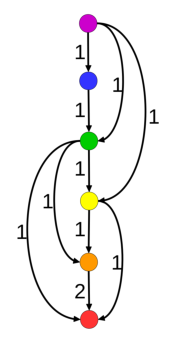
\includegraphics[width=.3\textwidth]{figures/dag.pdf}
    \caption{fig:DAGwidget}
    \label{fig:DAGwidget}
  \end{subfigure} 
  \caption{The widget}%\label{fig:example}
\end{figure}

\begin{figure}
 \begin{subfigure}[b]{0.45\textwidth}
    \centering
    \includegraphics[width=.5\textwidth]{figures/NST1An.pdf}
    \caption{fig:NSTwidget1}
    \label{fig:NSTwidget1}
  \end{subfigure}
  \quad
  \begin{subfigure}[b]{0.45\textwidth}
    \centering
    \includegraphics[width=.5\textwidth]{figures/NST2An.pdf}
    \caption{fig:NSTwidget2}
    \label{fig:NSTwidget2}
  \end{subfigure} 
  \caption{two possible changes}%\label{fig:example}
\end{figure}

\begin{figure}
 \begin{subfigure}[b]{0.45\textwidth}
    \centering
    \includegraphics[width=.5\textwidth]{figures/brick1NST.pdf}
    \caption{fig:DAGwidget1}
    \label{fig:DAGwidget1}
  \end{subfigure}
  \quad
  \begin{subfigure}[b]{0.45\textwidth}
    \centering
    \includegraphics[width=.5\textwidth]{figures/brick2NST.pdf}
    \caption{fig:DAGwidget1}
    \label{fig:DAGwidget2}
  \end{subfigure} 
  \caption{their DAG compression}%\label{fig:example}
\end{figure}


These \widgets can be pilled up as shown Figure
\ref{fig:empilement}. We will denote the tree obtained by pilling up
$n$ \widgets by $T_{n}$. The \widgets in $T_{n}$ are independent from
one another: it is possible to show that $T_{n}$ is
equidistant from every tree having the DAG compression of Figure
\ref{fig:NSTempilement} where every $A_{i}$ is either the DAG piece
Figure \ref{fig:DAGwidget1} or Figure \ref{fig:DAGwidget2}. We will
denote by $\mathcal{S}_{n}$ the set of these self nested trees. There
exists no tree closer to $T_{n}$ than these ones. %reference en annexe

\begin{figure}
 \begin{subfigure}[b]{0.45\textwidth}
    \centering
    \includegraphics[width=.5\textwidth]{figures/dag_brick.pdf}
    \caption{fig:empilement}
    \label{fig:empilement}
  \end{subfigure}
  \quad
  \begin{subfigure}[b]{0.45\textwidth}
    \centering
    \includegraphics[width=.5\textwidth]{figures/dagNST.pdf}
    \caption{fig:NSTempilement}
    \label{fig:NSTempilement}
  \end{subfigure} 
  \caption{pilling up the \widgets}\label{fig:example}
\end{figure}

To summarize, $T_{n}$ has exactly $2^{n}$ different NST and each one
of this self nested trees corresponds to an assignment of $n$
variables in $\{0;1\}$. As explained before, this could correspond to
the first step of a reduction of the NST problem. In order to complete
the reduction, we have to add \constraints. Adding \constraints means
modifing $T_{n}$ in function of the instance of INDEP-SET, in order to
obtain a tree $T$ closer to the self nested trees that correspond to valid
assignments of \variables for the instance of INDEP-SET. Given an
instance $\mathcal{I}$ of INDEP-SET, we will denote
by $\mathcal{S}_{\mathcal{I}}$ the subset of $\mathcal{S}_{n}$
constituted of the trees that correspond to valid assignments of
\variables in $\mathcal{I}$.
 
Let start with the first type of \constraint: if there is an edge
between $u$ and $v$ in the graph $G=(V,E)$ of $\mathcal{I}$, the
\variables represented by $u$ and $v$ cannot be both assigned to the
value 1. Given two vertices $u$ and $v$, if there is an edge between
$u$ and $v$, we have to modify $T_{n}$ to obtain $T$ such that $T$ is
closer to all the self nested trees of $\mathcal{S}_{n}$ where at
least one of the \widgets corresponding to $u$ and $v$ was modified
into Figure \ref{fig:DAGwidget2}, than the rest of
$\mathcal{S}_{n}$. By doing this modifications the NST of $T$ will be
the trees that correspond to a valid assignment of \variables.

The goal is to add successively this modifications for every edge in
$E$, and to reduce at every step the distance to the self nested trees
of $\mathcal{S}_{\mathcal{I}}$. By doing this modifications for every
edge in $E$, we should have applied all the \constraints of the first
type of the INDEP-SET problem and we would still have to find how to
translate the second one (the fact that only $k$ \variables can take
the value 1).

It appears that the modification for one edge has to reduce equally
the distance to all the trees of $\mathcal{S}_{\mathcal{I}}$, so that
the set of nearest self nested trees of $T$ is exactly
$\mathcal{S}_{\mathcal{I}}$. Otherwise, it is not possible to prove
the implication
$\omega_{\textsc{ NST }} = f(\omega_{\textsc{ Indep-Set }}) \in
Y_{\textsc{ NST }} \Rightarrow \omega_{\textsc{ Indep-Set }} \in
Y_{\textsc{ Indep-Set }}$

Unfortunately, the only modifications we found did not respect this
property. For this reason, we were not able to finish the proof with
this method.
 
\subsection{Last approach}

Since the second approch was not conclusive, I tried to approach the
problem form the other side: instead of trying to find the \widgets,
we will this time search to adapt the concept of \constraint to the
NST problem. 

As we said before, the \constraints are generally a sort of
translation from one problem to another of the difficulties. The issue
is that we do not know precisely at this point where the difficulty
truely lies in the NST problem. 

The algorithms proposed by C. Godin, P. Ferraro and R. Azais
\cite{godin, romain} to compute the NEST and the NeST rely on the fact
that since only addition or deletion operation are made, it is
possible to operate recursively on the DAG. More precisely, both
algorithm start by doing operations on the nodes of low height, in
order to make them all self-nested and isomorphic to one another,
recuresively use the changed nodes of low height to make the ones of
higher height alos isomorphic and self-nested. This method is possible
because only one type of operations is allowed.

Let illustrate on an example why this method does not seem to be
possible in the case of the NST problem. Let us consider the tree
Figure \ref{fig:treeexample}. Its NEST is shown Figure
\ref{fig:NESTexample}, its NeST is shown Figure \ref{fig:NeSTexample}.
Its NST is also its NEST. So far it does not seem particularly
difficult, the issue is that in tree Figure
\ref{fig:extendedexample} has for NST the tree
\ref{fig:extendedexampleNST}, where the subtrees of height 2 are
isomorphic to the tree Figure \ref{fig:NeSTexample} which is not the
NST of the subtrees of heigth 2 (isomorphic to \ref{fig:treeexample}).

The previous example highlights a sort of balance between two
irreconcilable goals: to be close to the initial tree $T$, the
subtrees of small height in the NST $S$ have to be close to the trees
of small height of $T$. But to make the higher nodes self-nested and
isomorphic to one anoher, it will sometimes be necessary to add whole
subtrees of smaller height. And therefore, the subtrees of small
height in $S$ also have to be of small size. This prevents us from
using a recursion from the bottom of the DAG to the top or in the
other direction. It prevents us from knowing where to start doing the
modifications: if we start with the upper part of the DAG, we will
need to know the exact size of the smaller subtrees to be able to
choose properly which operations have to be done; if we start with the
lower part of the DAG, we will have to know how many times the small
subtrees will be completely added in order to choose a self-nested
tree of small size yet close to the initial subtrees of small height.

The tree Figure \ref{fig:constraint} (that has the DAg compression shown
Figure \ref{fig:DAGconstraint}) is simple tree that depicts perfectly
this balance: the lower rhombus in the DAG needs to be modified in
odrer to become self-netsed, as well as the upper rhombus, but the
modifications made on any of them impacts the cost of the modifcation
made on the other one. 

This tree is at distance 12 from the self nested trees represented by
their DAG Figures \ref{fig:NST22}, \ref{fig:NST23} and \ref{fig:NST32}
and at distance 14 from the self nested tree Figure
\ref{fig:NST33}. The 3 first trees are the NST of the tree Figure
\ref{fig:constraint}. It is quite easy to see the two rhombus as
\widgets and assimilate them to \variables, that can take the values 2
or 3, depending on which one of the 4 self nested tree we consider.


\begin{figure}
 \begin{subfigure}[b]{0.45\textwidth}
    \centering
    %\includegraphics[width=.5\textwidth]{figures/dag_brick.pdf}
    \caption{fig:constraint}
    \label{fig:constraint}
  \end{subfigure}
  \quad
  \begin{subfigure}[b]{0.45\textwidth}
    \centering
    %\includegraphics[width=.5\textwidth]{figures/dagNST.pdf}
    \caption{fig:DAGconstraint}
    \label{fig:DAGconstraint}
  \end{subfigure} 
  \caption{}%\label{}
\end{figure}

\begin{figure}
 \begin{subfigure}[b]{0.22\textwidth}
    \centering
    %\includegraphics[width=\textwidth]{figures/dag_brick.pdf}
    \caption{fig:NST22}
    \label{fig:NST22}
  \end{subfigure}
  \quad
  \begin{subfigure}[b]{0.22\textwidth}
    \centering
    %\includegraphics[width=\textwidth]{figures/dagNST.pdf}
    \caption{fig:NST23}
    \label{fig:NST23}
  \end{subfigure}
  \quad
  \begin{subfigure}[b]{0.22\textwidth}
    \centering
    %\includegraphics[width=\textwidth]{figures/dag_brick.pdf}
    \caption{fig:NST32}
    \label{fig:NST32}
  \end{subfigure}
  \quad
  \begin{subfigure}[b]{0.22\textwidth}
    \centering
    %\includegraphics[width=\textwidth]{figures/dagNST.pdf}
    \caption{fig:NST33}
    \label{fig:NST33}
  \end{subfigure} 
  \caption{4 possibilites of variations}%\label{fig:example}
\end{figure}

The equal distance to the 3 first self nested tree is particularly
interessant because it is very similar to the \constraint of the
INDEP-SET problem (Figure \ref{tab:constraint})! As a short reminder,
the first type of \constraint for the INDEP-SET problem is that if two
vertices $u$ and $v$ are linked by an edge in $G$, the corresponding
\variables cannot be both set to 1.

We can see Figure \ref{tab:constraint} that the assignment of
\variables that corresponds to a valid independent set for the INDEP-SET
problem, are exactly the assignments of \variables that correspond to
the NST of the tree Figure \ref{fig:constraint}

\begin{figure}[h]
 \begin{subfigure}[b]{0.45\textwidth}
    \centering
    \begin{tabular}{|c|c|c|}
      \hline 
      $u$ & $v$ & \constraint \\
      \hline
      0 & 0 & respected \\
      0 & 1 & respected \\
      1 & 0 & respected \\
      1 & 1 & violated \\
      \hline
    \end{tabular}
    \caption{\Constraint of INDEP-SET}
    \label{tab:constIND}
  \end{subfigure}
  \quad
  \begin{subfigure}[b]{0.45\textwidth}
    \centering
    \begin{tabular}{|c|c|c|c|}
      \hline 
      $u$ & $v$ & distance & \constraint\\
      \hline
      2 & 2 & 12 & respected \\
      2 & 3 & 12 & respected \\
      3 & 2 & 12 & respected \\
      3 & 3 & 14 & violated \\
      \hline
    \end{tabular}
    \caption{\Constraint of NST}
    \label{tab:constNST}
  \end{subfigure} 
  \caption{Constraints}\label{tab:constraint}
\end{figure}

% \subsection{Intuition guiding the researches}

% \begin{itemize}
% \item Approche 1: se familariser avec le problème en se restraignant à
%   un sous-ensemble et montrer que déjà là c'est dur. Risque possible:
%   se restraindre à un sous-ensemble où en fait, c'est polynomial. Ça
%   permet quand même en général de mieux comprendre son problème.
% \item Approche 2: Preuve de NP-complétude à base de \widget,
%   i.e., de structures particulières que l'on peut combiner
%   astucieusement pour exprimer les \constraint du problème
%   auquel on cherche à se réduire.
% \item Approche 3: Trouver un graphe qui paraisse particulièrement
%   difficile.
% \end{itemize}

% In this section, I illustrate the second approach, where \widgets
% are built and linked to each others through \constraints. 

% Let us begin with the proof of the reduction from 3-SAT to INDEP-SET
% \cite{polytech}. As a brief reminder:
% \begin{definition}[3-SAT]
  
% \end{definition}

% \begin{definition}[INDEP-SET]
  
% \end{definition}
% \begin{figure}

%   \centering
  
%   \caption{3SAT reduction}
%   \label{fig:3sat}
% \end{figure}

% %%%%%%%%%%%%%%%%%%%%%%%%%%%%%%%%%%%%%%%%%%%%%%%%%%%%%%%%%%%%%%%%%%%%%%%%%%%%
% \noindent\hrulefill

% In the reduction proposed by Garey and Johnson\cite{garey}, the image
% instance of INDEP-SET is built in two steps: the first one consists in
% defining triangles that correspond to each clause of the initial
% instance of 3-SAT (see Figure\ref{fig:3sat}); the second one consists
% in adding edges that link the nodes of the \widgets that are labeled
% with the negation of the same variable of 3-SAT. One way of
% interpreting this division in two steps is to consider the triangle
% \widgets as \variables that can take three different values (the
% \variable term here should not be confused with the variable of the
% 3-SAT problem). 

% These three values are the label of three nodes of the
% triangle, and the value taken by the variable is the label of the node
% taken in the set of vertices of INDEP-SET.

% The edges linking the nodes are representing
% the constraints of the first problem

% Furthermore, we can observe that generally, the construction of the
% image instance seems to be combination of two different things: a part
% that reflects only the number of variables in the instance of the
% first problem and a part reflecting the links and constraints that
% they have with one another.  For example, in the proof of the
% reduction from 3-SAT to INDEP-SET \cite{polytech}, the first part
% consists in the triangles corresponding to each clause of the initial
% instance, and the second to the edges linking the nodes such as one is
% labeled with the negation of the other. In the proof of the reduction
% from VERTEX-COVER to HAMILTONIAN-CYCLE \cite{polytech}, the first part
% consists in the 12 nodes widgets corresponding to each edge of the
% initial graph, and the second part consists in the way they are linked
% to one another to form the image graph.

% We can also observe that in the first part, a piece of the image
% instance corresponds to each variable of the initial
% instance. Moreover, this piece of the image instance is very
% restrictive and can be used in a solution only in a few (2 or 3 most
% of the time) different ways. For example in the proof of the reduction
% from VERTEX-COVER to HAMILTONIAN-CYCLE \cite{polytech}, the widgets
% can either be visited in one pass or in two.

% Furthermore the way these pieces are used is completely independant
% until the second part corresponding to the constraints between the
% variables is added.

% \subsection{Trees of height 2 without variation of the height}
% The edit distance with constraint of K.Zhang being slightly difficult
% to manipulate, we will use a far more restrictive variant in this
% section: only leaves (and not internal nodes) can be added or
% deleted. More precisely, if $u$ is an ancestor of $v$ in $T$ and
% $v \in V'_{1}$ then $u \in V'_{1}$.

% In this section we present a polynomial algorithm computing the
% nearest self-nested tree of height 2 to a tree of height 2.

% \subsection{Trees of height 2 with variation of the height}
% In this section, we present a polynomial algorithm computing the nearest
% self-nested tree to a tree of height 2.

% \subsection{Family of bricks}
% In this section, we present a family of trees that could be used as
% the first part of the reduction to represent the variables of the
% initial instance.